% Rafael Sartori M. dos Santos, 186154
\documentclass[brazilian,a4paper,twocolumn]{article}

% Título
\title{MC920 -- Trabalho 5}
\author{Rafael Sartori M. Santos, 186154}
\date{21 de novembro de 2019}

% Configuração do documento
\setlength{\parskip}{3pt}
\usepackage[utf8]{inputenc} % tipo de documento UTF-8
\usepackage{mathtools} % permitir expressões matemáticas
\usepackage{breqn} % equações quebradas em várias linhas automaticamente
\usepackage{babel} % configuração da lingua portuguesa
\usepackage{caption} % para legenda de tabelas e figuras
\usepackage[
    pdfauthor={Rafael Sartori M. Santos},
    pdftitle={Trabalho 5 -- MC920},
    pdfproducer={LaTeX (texlive) com hyperref},
    hidelinks
]{hyperref} % para links externos (href)
\usepackage{cleveref} % para referenciar tabelas e figuras melhor
\usepackage{indentfirst} % indentação de todo primeiro parágrafo
\usepackage{graphicx} % para adicionar imagens
\graphicspath{{../imgs_in/}{../imgs_out/}} % atalho para o caminho das imagens
\usepackage{float} % para fixar posição de imagens
\usepackage{subcaption} % para imagens ficarem lado a lado
% Usamos geometry pois dá mais espaço que fullpage
%\usepackage{geometry} % alterar geometria do papel
%\geometry{a4paper,left=1.7cm,right=1.7cm,top=1cm,bottom=2.0cm} % menor margem
\usepackage{fullpage} % utilizamos uma versão com menos espaçamento nas bordas
\usepackage{verbatim} % pacote para incluir arquivos em verbatim
\usepackage{mdframed} % para enquadrar coisas
\usepackage[bitstream-charter]{mathdesign} % Mudamos a fonte para Charter BT
\usepackage[T1]{fontenc} % Mudamos a fonte para Charter BT

% Início do documento
\begin{document}

\maketitle


\section{Introdução}

    O objetivo do trabalho é avaliar o procedimento PCA (\textit{Principal Component Analysis}) como efetivo método de compressão de imagens através da redução de componentes menos significativos.

    Faremos isso através de um programa Python que utiliza as bibliotecas \href{https://opencv.org/}{\emph{OpenCV}}, \href{https://numpy.org/}{\emph{NumPy}} e padrão.


\section{Metodologia}

    Analisaremos a compressão feita com a redução de componentes dados pelo PCA nas imagens dadas pelo professor no enunciado do trabalho e em uma imagem de grande dimensão (comparada às outras) capturada por um celular comum moderno.

    Todas as imagens utilizadas estavam no formato \texttt{PNG}, como especificado no enunciado, para não serem afetadas pela compressão com perdas de outros métodos. Durante o desenvolvimento do projeto, sobreescrevemos as imagens originais utilizando a biblioteca \emph{OpenCV} (a mesma que utilizaremos para salvar as imagens alteradas), de forma a minimizar os efeitos das diferentes implementações do formato \texttt{PNG}.

    Começamos o programa descrevendo diversas opções de entrada para o usuário: qual imagem será utilizada, o parâmetro $k$ para redução de componentes, onde salvaremos a imagem final, o relatório (em texto) de análise da compressão e ainda se utilizaremos a implementação para SVD (\textit{Singular Value Decomposition}, uma das maneiras de se fazer PCA) já feita de \emph{NumPy} ou, caso contrário, se utilizaremos a nossa implementação.

    Utilizando essas opções, abrimos a imagem através de \emph{OpenCV}, isolando as camadas de cores para serem tratadas individualmente e as transformando em vetor de pontos flutuantes.

    \subsection{Utilizando SVD de \emph{NumPy}}

        Na implementação utilizando SVD de \emph{NumPy}, fazemos a decomposição e, posteriormente, pegamos apenas os $k$ primeiros componentes mais significativos para refazer a imagem. Isso pode ser visto na \cref{eq:pca-svd}, considerando $g$ a imagem final e $f$, a inicial.

        \begin{subequations}
            \label{eq:pca-svd}
            \begin{equation}
                \label{eq:pca-svd-decomposicao}
                U, D, V^T = \texttt{svd}(f)
            \end{equation}
            \begin{equation}
                \label{eq:pca-svd-recombinacao}
                g = U_{[:, 0:k]} D_{[0:k]} V^T_{[0:k, :]}
            \end{equation}
        \end{subequations}

        Na \cref{eq:pca-svd-decomposicao}, \emph{NumPy} já ordena decrescentemente o resultado de SVD, o que é mais amigável as aplicações que utilizam isso para fazerem PCA. Desta forma, é bem rápido e fácil de implementar um algoritmo de compressão que utiliza PCA, mas não vemos com detalhes as operações realizadas nem a interpretação não usual da imagem como componentes.

    \subsection{Implementação própria}

        Já na implementação própria de PCA, ao contrário, fazemos a compressão em detalhes, podemos entender melhor a análise interpretando a matriz da imagem como um vetor de informações, onde cada linha é um componente e cada coluna diferentes atributos desse componente.

        Com a imagem inicial $X$, na \cref{eq:pca-1}, removemos de cada componente a média dos atributos (representada na matriz $\overline{X_j}$), de forma a obtermos uma média zero individualmente. Com isso, podemos obter a matriz de covariância $X_n$, como em \cref{eq:pca-covariancia}.

        \begin{subequations}
            \label{eq:pca-1}
            \begin{equation}
                \label{eq:pca-media}
                X_n = X - \overline{X_j}
            \end{equation}
            \begin{equation}
                \label{eq:pca-covariancia}
                \Sigma = X_n X_n^T
            \end{equation}
        \end{subequations}

        Com a matriz de covariância da \cref{eq:pca-covariancia}, encontramos e ordenamos os autovetores decrescentemente pelos seus autovalores na \cref{eq:pca-2}. Disso, isolamos os $k$ primeiros componentes dos autovetores.

        \begin{subequations}
            \label{eq:pca-2}
            \begin{equation}
                \label{eq:pca-autovalorvetor}
                \lambda, V = \texttt{sort}(\texttt{eig}(\Sigma))
            \end{equation}
            \begin{equation}
                \label{eq:pca-autovetor-k}
                V_k = V_{[:, 0:k]}
            \end{equation}
        \end{subequations}

        Utilizando os $k$ primeiros componentes, refazemos a matriz original na \cref{eq:pca-3} utilizando os $k$ primeiros autovetores e a matriz sem as médias, somando as médias removidas e finalmente produzindo a imagem final $X_f$.

        \begin{subequations}
            \label{eq:pca-3}
            \begin{equation}
                \label{eq:pca-saida}
                \hat{X} = V^T_k X_n
            \end{equation}
            \begin{equation}
                \label{eq:pca-recomposicao}
                X_f = (V_k \hat{X}) + \overline{X_j}
            \end{equation}
        \end{subequations}


    \subsection{Avaliando resultados}

        Agora, com as duas formas de se produzir uma imagem utilizando menos componentes, podemos avaliar a compressão. Para isso, salvamos cada imagem utilizando \emph{OpenCV}, calculamos a taxa de compressão e RMSE (\textit{Root mean square error}). Esses dados são impressos em um arquivo e podem ser comparados apenas dentro de uma mesma imagem (devida natureza de RMSE).

        Os testes foram automatizados através de um \textit{script} \texttt{bash}. Fazemos para cada imagem alguns valores de $k$: 32, 64, 128, 192 e 256, produzindo uma imagem de saída e um relatório diferente.


\section{Resultados}

    % falar de modo gerão da compressão e resultados

    % apresentar imagens versão -menor

    Como explicitado em aula, podemos comprovar a dificuldade para escolher um valor $k$. Há imagens em que visualmente não podemos notar artefatos com $k$ pequeno e outras que fazem muita diferença, mesmo em dimensões parecidas. Podemos perceber isso na comparação das imagens \texttt{monalisa} e \texttt{watch-menor} na \cref{fig:comparativo-watch-monalisa}, cujas dimensões são parecidas e número de \textit{pixels} diferem em cerca de apenas 2 mil.

    \begin{figure}[H]
        \centering
        \begin{subfigure}{0.23\textwidth}
            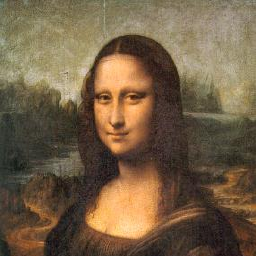
\includegraphics[width=\textwidth,keepaspectratio]{monalisa}
            \caption{\texttt{monalisa} original}
            \label{fig:monalisa-original}
        \end{subfigure}
        \begin{subfigure}{0.23\textwidth}
            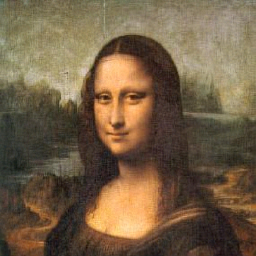
\includegraphics[width=\textwidth,keepaspectratio]{monalisa-64}
            \caption{\texttt{monalisa} $k=64$}
            \label{fig:monalisa-64}
        \end{subfigure}

        \begin{subfigure}{0.23\textwidth}
            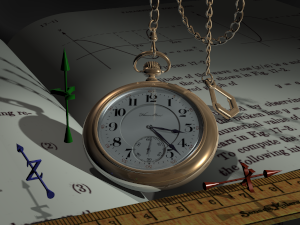
\includegraphics[width=\textwidth,keepaspectratio]{watch-menor}
            \caption{\texttt{watch-menor} original}
            \label{fig:watch-menor-original}
        \end{subfigure}
        \begin{subfigure}{0.23\textwidth}
            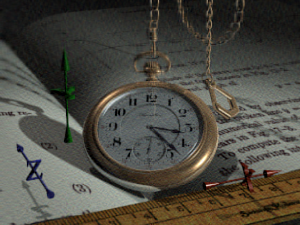
\includegraphics[width=\textwidth,keepaspectratio]{watch-menor-64}
            \caption{\texttt{watch-menor} $k=64$}
            \label{fig:watch-menor-64}
        \end{subfigure}

        \caption{Comparativo entre duas imagens de dimensões próximas}
        \label{fig:comparativo-watch-monalisa}
    \end{figure}


\section{Conclusão}



\end{document}
